
\documentclass[]{article}
\usepackage{graphicx}
\usepackage{color}
\usepackage[parfill]{parskip}

%opening
\title{MetaTracts - A Method for Robust Extraction and Visualization of Carbon Fiber Bundles in Fiber Reinforced Composites: Rebuttal}
\author{}

\begin{document}
\noindent

\maketitle
We thank the reviewers for their reviews of the submitted manuscript, in order to address the raised queries we carefully re-worked and improved the manuscript, improved some figures, included additional explanations, and extended supplementary material. This document describes a summary of the introduced improvements. The summary review mentioned three main issues: 
\textbf{\textit{
\begin{enumerate}
	   \item  Visualization of more datasets, particularly, the ones, as R1 has
	   mentioned with crossings at other angles.
	   \item Effects of choice of length in MetaTract generation.
	   \item Performance studies and limitations.
\end{enumerate}
}}
We fully dedicated ourselves to address these comments and incorporated the following changes:
\begin{enumerate}
	\item {Due to the manufacturing process, a vast majority of composites have bundles crossing at ~90 degree angles. With the separation factors being widths, spacings and compactness of fiber bundles. These variations are well represented in our data sets: total of three in the original submission. We present evaluation of MetaTracts for datasets D1 and D2 in the main manuscript. Additionally applicability for dataset D3 and glass fiber reinforced dataset is presented in the supplimentary material due to space constraints. Therefore we argue that the technique is useful and applicable to a range of various composite polymers. Providing additional datasets is unfortunately not possible given the time constraints of the minor revision. 
		
		In dataset 1, Figure~\ref{fig:angle_bundles}f, bundles 7,10 and 6 show  bundles which  though parallel differ in angle and bundle width. It is a common example of variations in the datasets which we extract accurately. 
		
		During additional experiments, we did apply our technique to a different class of fibers where the individual fibers are clearly visible, namely the glass-fibers. We have added the results to the supplementary section. 
		\begin{figure}
			\centering
			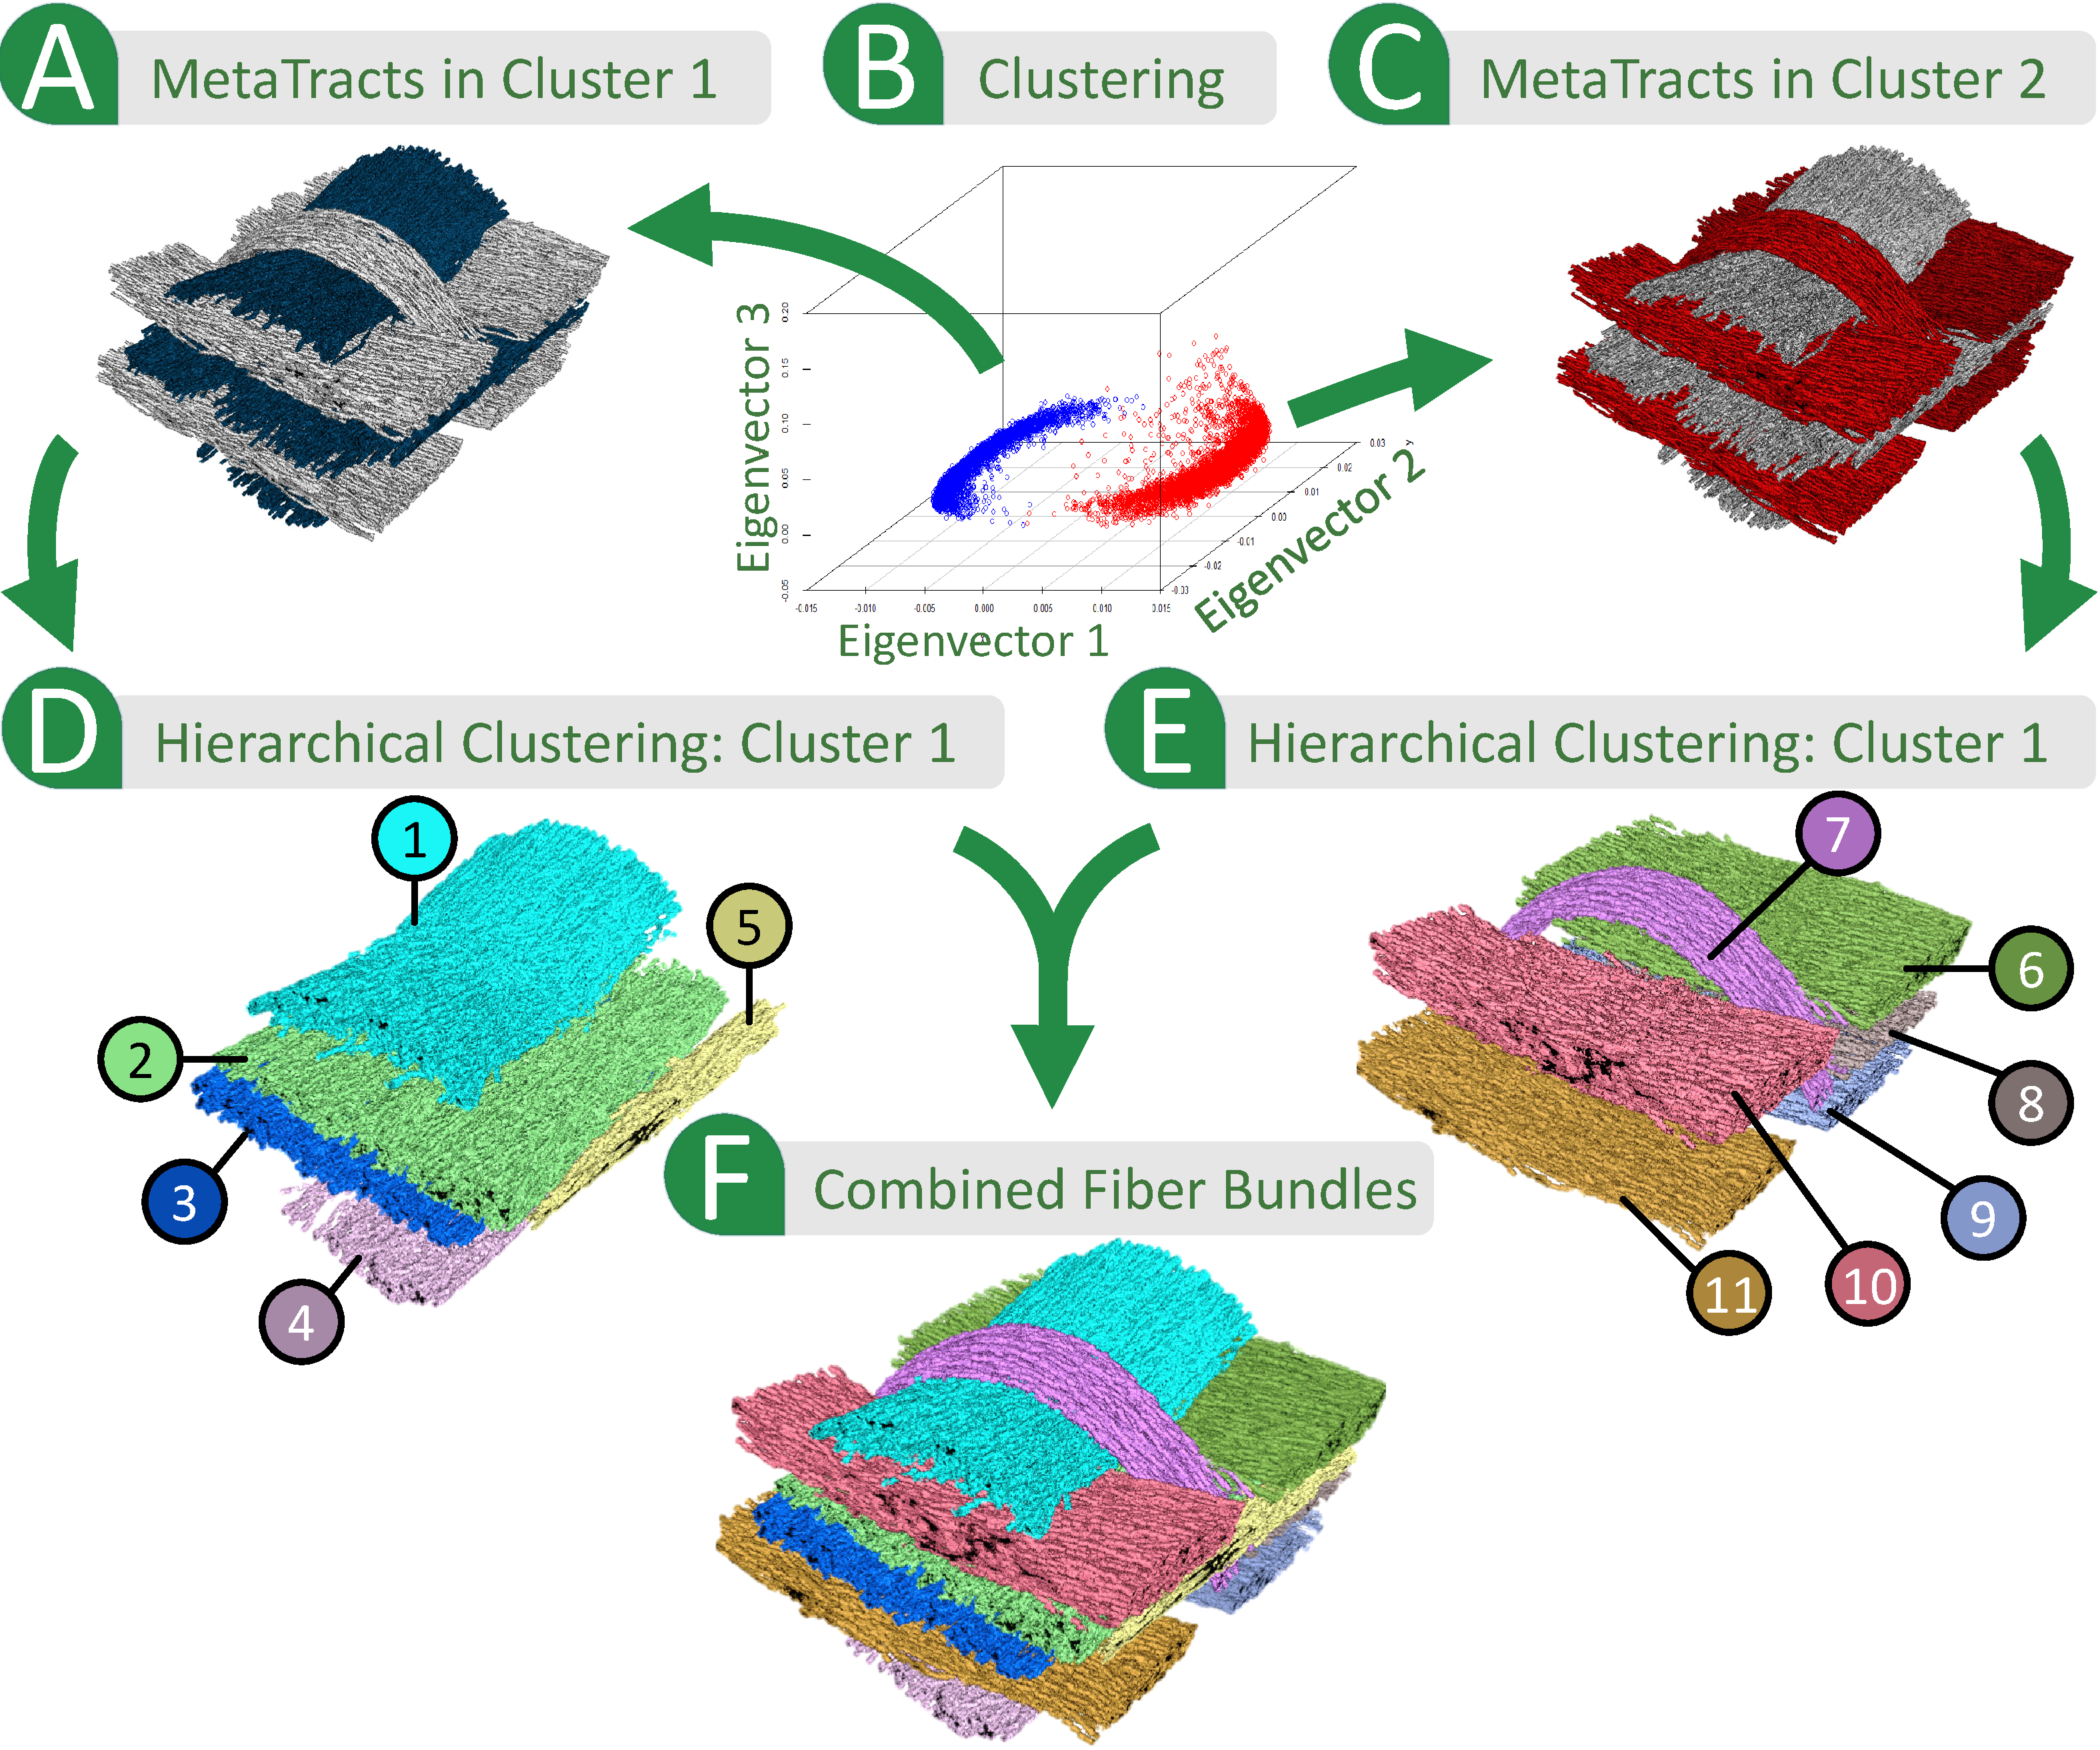
\includegraphics[width=0.7\linewidth]{images_pvis/clustering.pdf}
			\caption{Fiber bundles extraction}
			\label{fig:angle_bundles}
		\end{figure}}
		\item {
			We clarified the effects of choice of length and radius of MetaTracts cylinders in the paper: 
			``The length and the radius parameters for the cylinders of MetaTracts decide how coarse the fiber cylinders are. These are dependent on the underlying fiber characteristic and the weaving pattern. Larger cylinders will handle noisy local orientation better as it inspects a higher number of candidate points to extend the fiber. We used 10.00 and 2.00 for length and radius (measured in grid voxel size), respectively for all tests.  
			Simpler geometry (example dataset 2) was experimentally found to handle larger cylinders better.''
			
			Reviewer 3 and  4, asked  about the effect of the length threshold ``$\eta$".  ``$\eta$" on how quickly the hierarchical clustering converges. We mention in the manuscript that our experimental studies concluded that the length threshold choice of 0.3 to 0.6 gave qualitatively similar results. Quantitatively in our  tests $1.2\% - 5\%$ of fibers (total number of fibers $\sim$10000)were removed, while quantitatively small, without removing these clusters are difficult to separate. These experimental results were included in the paper.
			}
			\item{
				We have added a limitations section to the paper. We also detailed the approximate times of MetaTracts computation for our datasets in the Experimental Results section of the paper. Unfortunately the full scale performance study was not possible due to the time constraints of the minor revision. Additional difficulty of obtaining the detailed performance numbers is that it would require the access to workstations which are actively used and regularly occupied by other researchers and developers. Therefore only the reasonable round-ups of the performance and computation run-times are presented.
				}
\end{enumerate}
   
 The remainder of this document addresses comments and remarks raised by individual reviewers.

\section{Reviewer 1}

\textbf{\textit{
Q1. A new variable, reliable Hessian, is defined and it is stated that $R_{H}$ is similar to the "vesselness".  Later on, the authors claim "the utility of the vesselness is a little different from our framework". Matching term by term between the definitions of "vesselness" and $R_{H}$, they are the same. The authors are encouraged to state clearly the originality and contribution of $R_{H}$.
}}


A1. Reliable Hessians is computed exactly equivalently to Vesselness for a single scale (Firangi et al.~\cite{Frangi1998}). We have  updated the corresponding sentence in the paper to reflect this information. We explain further about the utility being different.

A common approach and one utilized by the Frangi et al.~\cite{Frangi1998}, is to consider the Taylor series expansion in the neighborhood of point $x$ in an image as.
\begin{equation}
f(x) = \sum_{i=0}^{\infty}\frac{f^{(i)}(0)}{i!}x^{i}
\end{equation}
The expansion often is approximated till the second order (Hessian). In particular the hessian maps a  neighborhood  centered about $x$ onto an ellipsoid  whose axes are along the directions given by the eigenvectors of the Hessian and the corresponding axis' semi-lengths are the magnitudes of the respective eigenvalues. Vesselness measure as described in the paper takes into account geometric ratios based on this and acts as a filtering process which searches for geometric structure that can be tubular. Figure~\ref{fig:Vesselness} shows results from Frangi et al.~\cite{Frangi1998} paper. Others including Sato et al.~\cite{Sato1997} have used the eigen decomposition to filter images.

As mentioned in the paper, we do not have clear tubular structures embedded in a dark contrast matrix such as in blood vessels ( Figure~\ref{fig:data-char-rebuttal} shows the data characteristics for our case.). Instead  the utility of $R_{H}$ is  to associate each grid location with a reliability measure for the local orientation as given by the  principal eigenvector. We use this orientation vector to create MetaTracts.
\makebox[\linewidth]{\rule{0.25\textwidth}{0.4pt}}

\begin{figure}
\centering
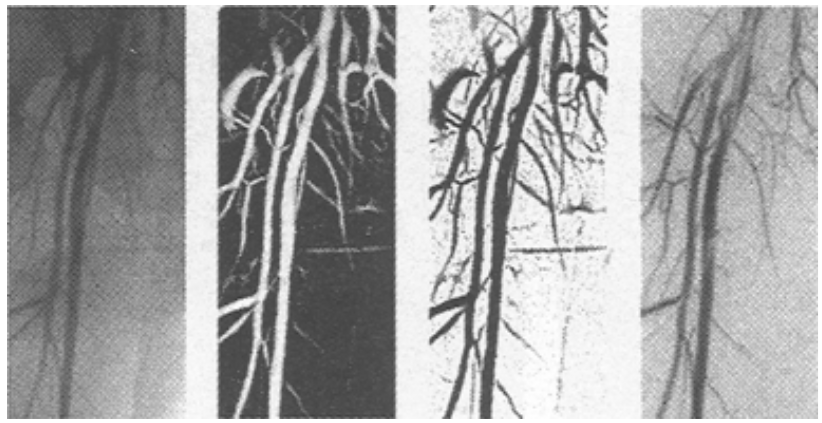
\includegraphics[width=0.7\linewidth]{images_pvis/Vesselness}
\caption{Left: Xray image of vasculature, middle-left: calculated vesselness of the left image, middle-right: calculated vesselness after inversion of the grey-scale map. Right image after subtracting reference from left image.}
\label{fig:Vesselness}
\end{figure}

\begin{figure}[tb]
	\centering
	%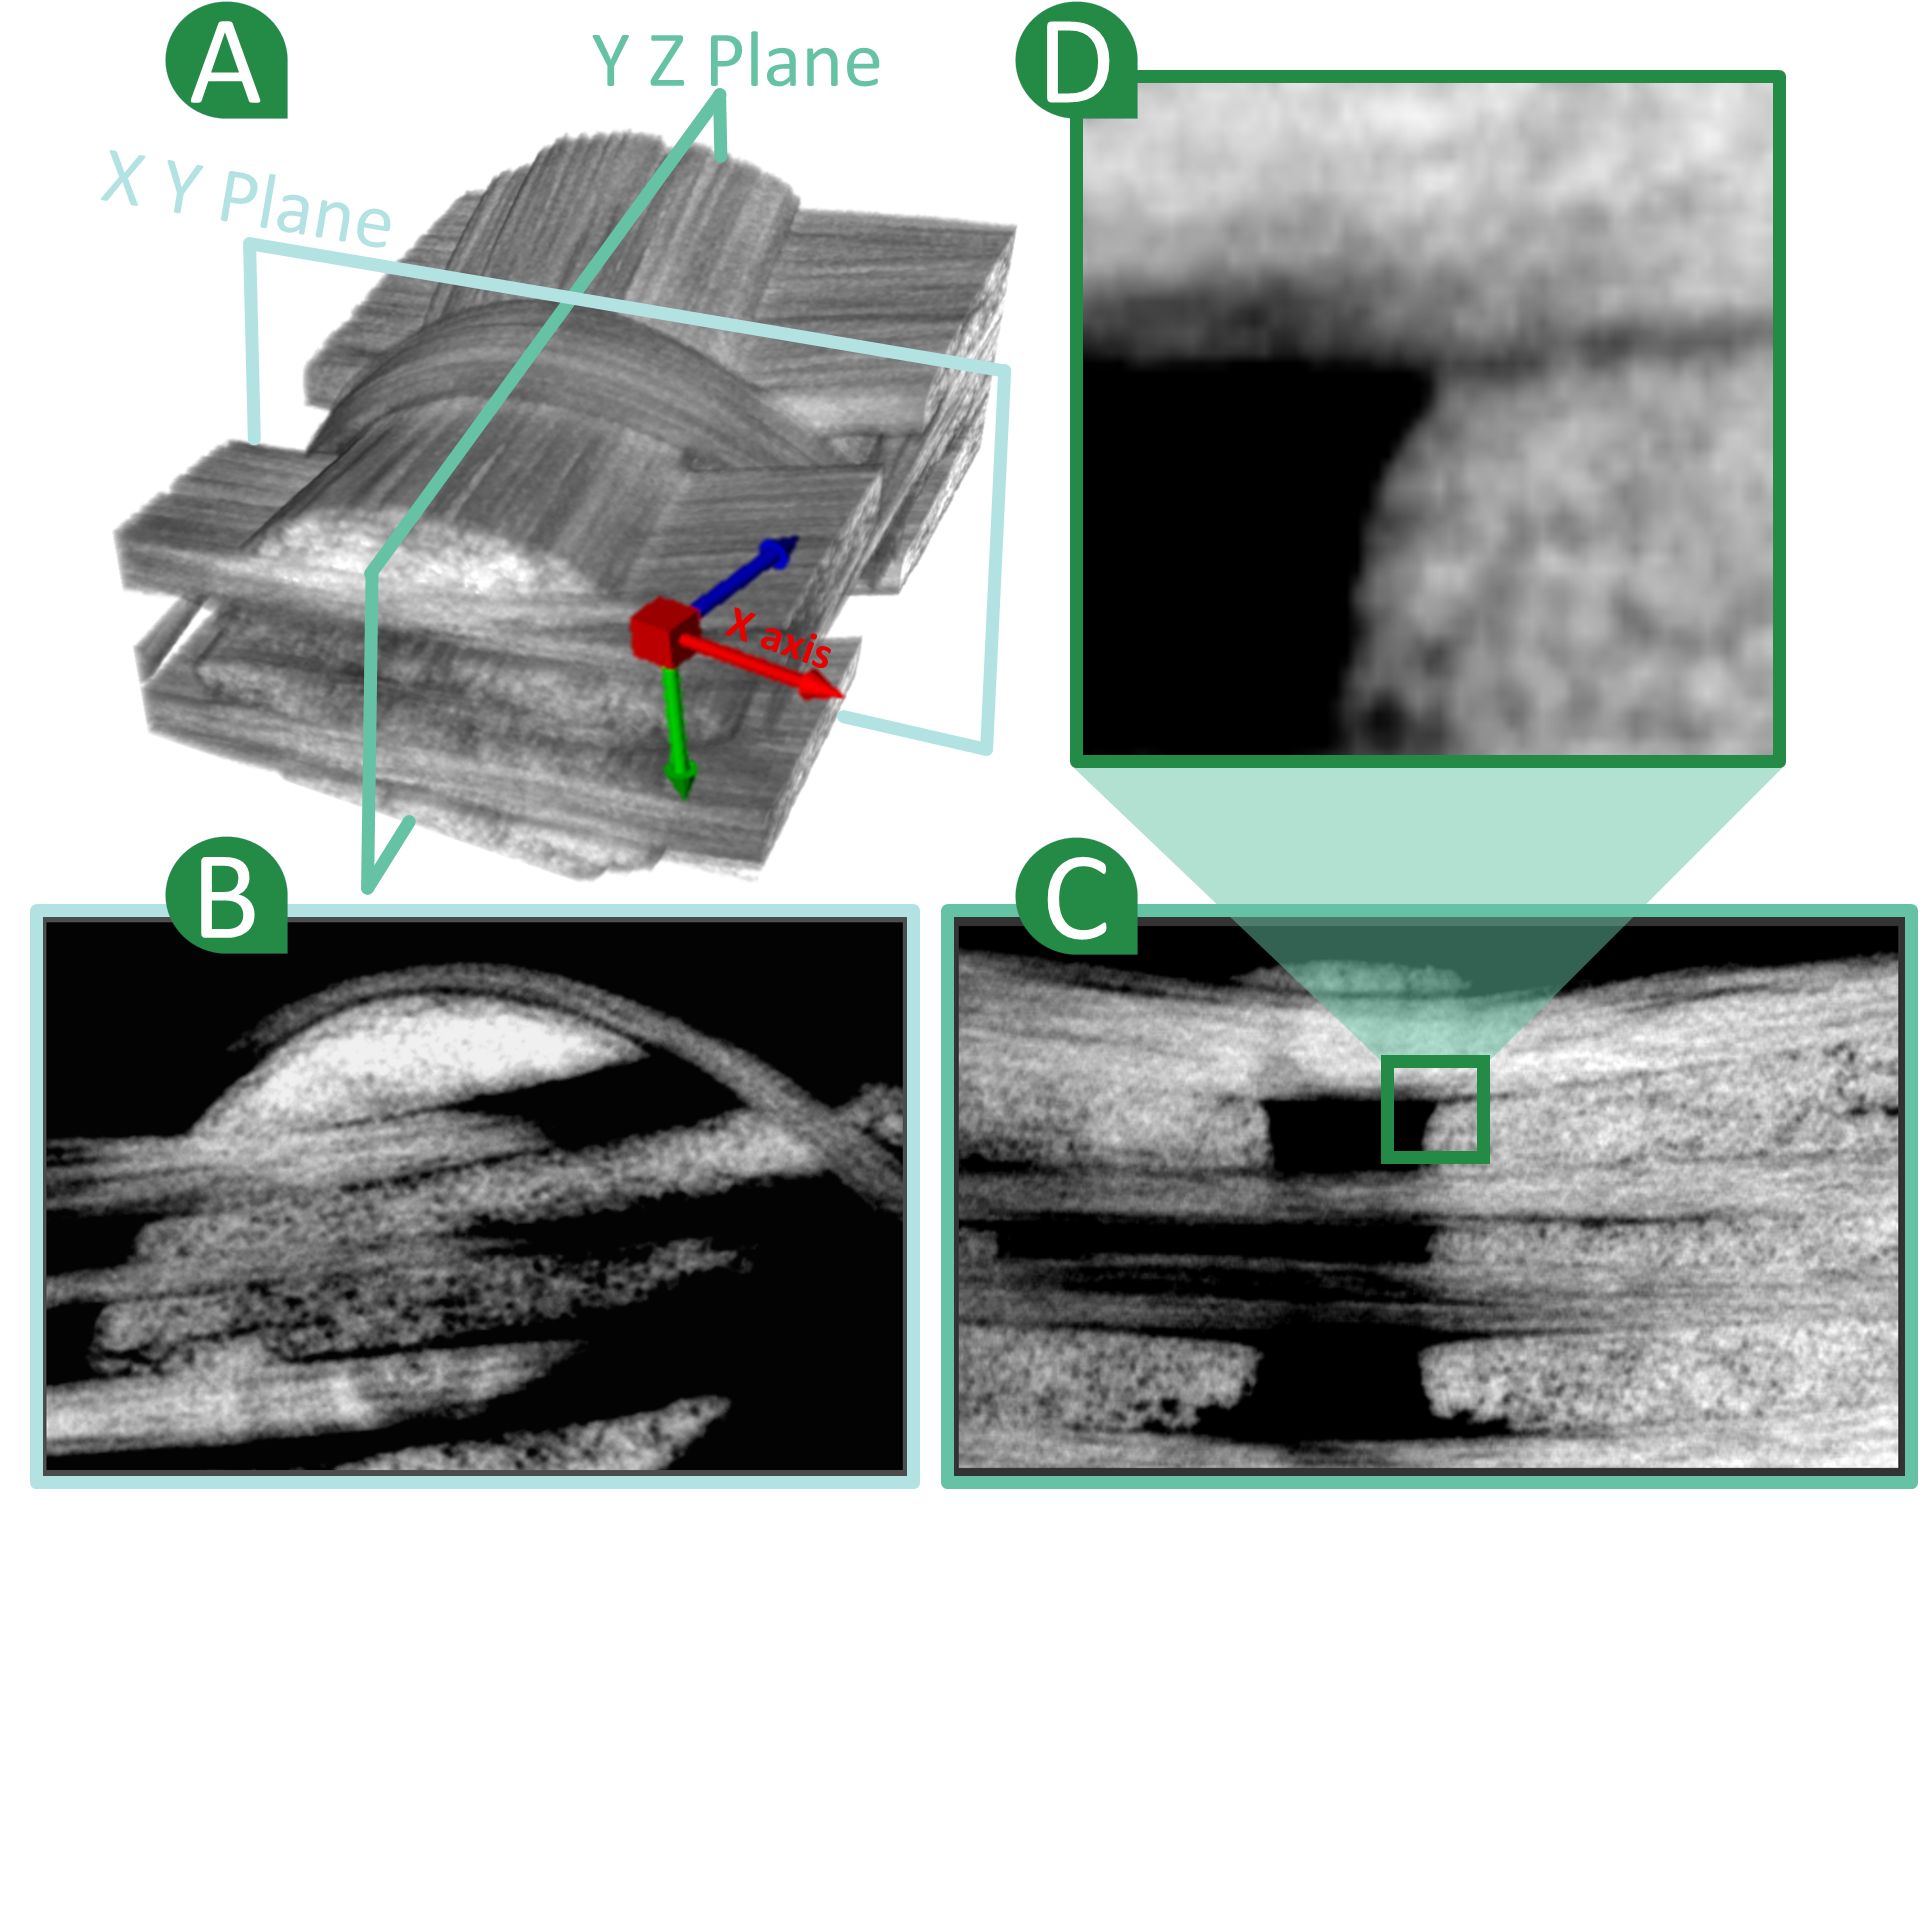
\includegraphics[width=0.5\textwidth, trim = 0mm 110mm 0mm 0mm, clip,]{images_pvis/figure1}
	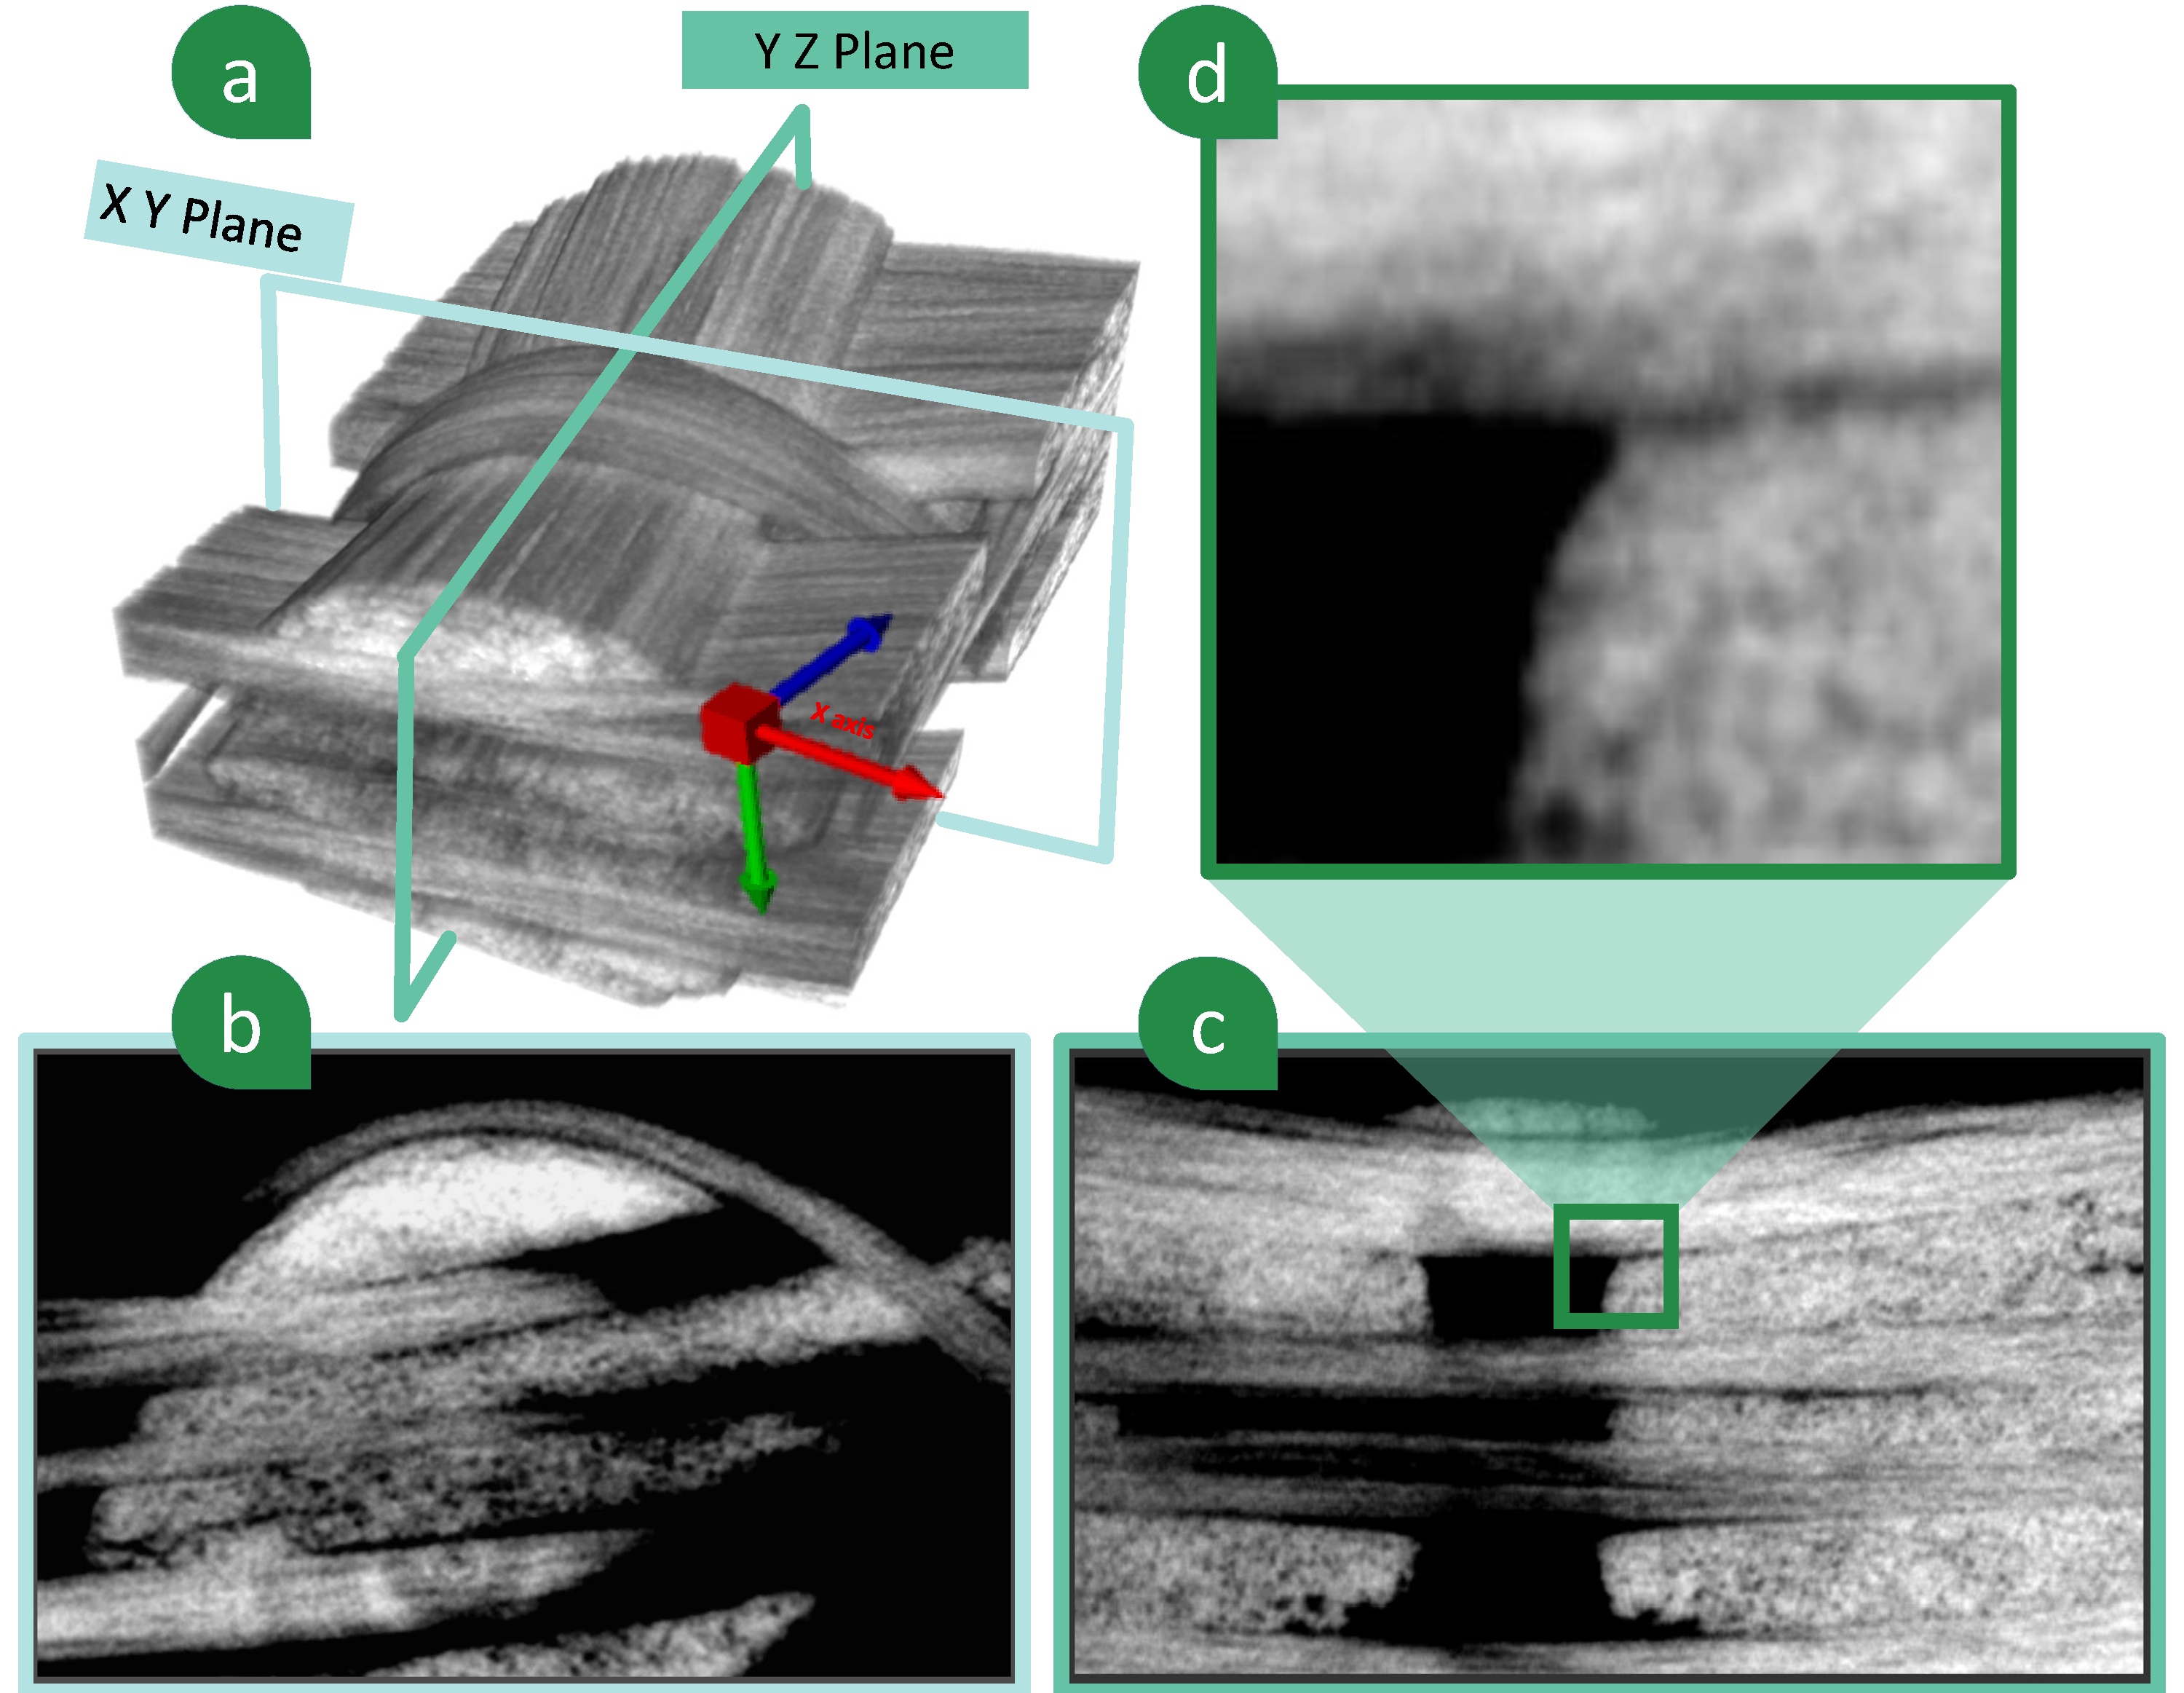
\includegraphics[width=\linewidth]{images_pvis/data-char.pdf}
	\caption{Data characteristics: (a) Rendering of the data. (b) 2D slices along the X-axis and (c) 2D slice along the Z-axis. (d) Magnified region marked in green square (c). Multiple fiber bundles cross and are indistinguishable by visual inspection alone. }
	\label{fig:data-char-rebuttal}
\end{figure}


\textbf{\textit{
Q2. In the examples presented, it seems only one type of composite was studied. For instance, there is no example showing a composite with fiber bundles that cross each other at an angle $<$ 90 degrees. When two bundles are almost parallel, will the current algorithm be sufficient to separate them apart? The authors are encouraged to provide more than one fiber configurations.
}}


A2. Please see answer 1 to the summary review and the extended supplementary material.  

\makebox[\linewidth]{\rule{0.25\textwidth}{0.4pt}}


\textbf{\textit{
Q3. All clustering was done in R. The letter R is not explained.
}}


A3. R is a free software environment for statistical computing and graphics. This explanation is now added to the paper.

\makebox[\linewidth]{\rule{0.25\textwidth}{0.4pt}}

\section{Reviewer 2}

\textbf{\textit{
Q1. I feel the background section could be improved. Why the orientation and weaving patterns of fibers indicate the strength of the material, and thus why the trouble to scan the materials, extract the fibers and visualize them. The paper gives some relatively high-level description of this but more background would be appreciated.
}}



A1. We modified the related works section.

\makebox[\linewidth]{\rule{0.25\textwidth}{0.4pt}}


\textbf{\textit{
Q2. It seems to me that the extracted fibers may not be real fibers. Is this
true? If so, how well can one trust the weaving patterns extracted based
on the imaginary fibers?
}}


A2. Yes, the extracted fibers cannot be mapped to real fibers. One of our main goals is to move away from extraction of individual fibers and work instead on direct reconstruction of bundles. These design decisions adheres to extracting reliable bundles directly from the images.
Developing methods which can precisely compute the deviations from original bundles remains a future direction of the project. We did experiment with glass fibers (see supplemental section) where the individual fibers are clearly separated, and proved as a sanity check that the MetaTract technique does extract correct fibers.
 
\makebox[\linewidth]{\rule{0.25\textwidth}{0.4pt}}


\textbf{\textit{
Q3. The authors claim that their method can deal with low resolution data.
But this might be in the eyes of the beholders, since in my opinion the example data in the paper all have fairly high resolutions. Perhaps a comparison with a really high resolution data using this method and other existing methods could diffuse the doubt.
}}


A3. In the context of this work by low resolution we intend situations when resolving individual fibers is not possible. We state this in the paper. Please look at the supplementary section on glass fibers as an example of high-resolution data.

\makebox[\linewidth]{\rule{0.25\textwidth}{0.4pt}}

\section{Reviewer 4}

\textbf{\textit{
Q1. In Section 5.1, k-means is applied to the m-dimensional space using
Euclidean distance, i.e., each dimension is considered equally important.
Is that really the case when they represent eigenvectors?
}}


A1. Belkin  and Niyogi's~\cite{Belkin01} laplacian eigenmaps embeds the high dimensional data ( represented as a graph ) into a low dimensional space where the Euclidean distance approximates the distances in higher dimension space. For such reason, Eigen embedding for dimensionality reduction has become quiet popular and has found favor in tackling a variety of problems. Empirically the K-means for orientation clustering provided us with excellent results. The major orientations are limited by the inherent characteristics of our data set and this also plays a role in Laplacian embedding followed by k-means giving us such good results. A formal proof is not provided due to the strict space constraints.
 
\makebox[\linewidth]{\rule{0.25\textwidth}{0.4pt}}


\textbf{\textit{
Q2. In Section 5.2, the authors mention that they remove short Meta Tracks.
How much data is thrown away here? Can examples be provided to get a
better understanding?
}}


A2. Please see the answer 2 to the summary review.

\makebox[\linewidth]{\rule{0.25\textwidth}{0.4pt}}


\textbf{\textit{
Q3. What are the limitations of the approach? Are there data sets where the
method fails?
}
}

A3. We have added a ``Limitations and future work" Section to the end of the paper. We cite it here for completeness:

A key assumption of the method is ``connectivity'' (Sec. Data Characteristic).
If the ``connectivity'' is not satisfied due to noise in the image, the then MetaTracts will be inaccurate. 
The clustering process also assumes that the fiber bundles have a minimum width. 
\bibliographystyle{abbrv}
%%use following if all content of bibtex file should be shown
%\nocite{*}
\bibliography{xBundle}
\end{document}
